%%%%%%%%%%%%%%%%%%%%%%%%%%%%
% CHAPTER 7 - DISCUSSION of STUDY/EVAL METHODS
%%%%%%%%%%%%%%%%%%%%%%%%%%%%
%%%%%%%%%%%%%%%%%%%%%%%%%%%%%%%%%%%%%%%%%%%%%%%%%%%%%%%%%%%%%%%%%%%%%%%%%%%%%%%%%%%%%%%%%%
% Richard Boardman PhD Thesis: Improving Tool Support for Personal Information Management
%%%%%%%%%%%%%%%%%%%%%%%%%%%%%%%%%%%%%%%%%%%%%%%%%%%%%%%%%%%%%%%%%%%%%%%%%%%%%%%%%%%%%%%%%%

%%%%%%%%%%%%%%%%%%%%%%%%%%%%%%%%%%%%%%%%%%%%%%%%%%%%%%%%%%%%%%%%%%%%%%%%%%%%%%%%%%%%%%%%%%
% NATBIB NOTES
%%%%%%%%%%%%%%%%%%%
%\citet{jon90}                ->    Jones et al. (1990) 
%   \citet[chap.~2]{jon90}       ->    Jones et al. (1990, chap. 2)
%   \citep{jon90}                ->    (Jones et al., 1990) 
%   \citep[chap.~2]{jon90}       ->    (Jones et al., 1990, chap. 2) 
%%%%%%%%%%%%%%%%%%%%%%%%%%%%%%%%%%%%%%%%%%%%%%%%%%%%%%%%%%%%%%%%%%%%%%%%%%%%%%%%%%%%%%%%%%

\newpage
%%%%%%%%%%%%%%%%%%%%%%%%%%%%%%%%%%%
\section{Methodological Recommendations}
\label{discussion:methodological-discussion}
%%%%%%%%%%%%%%%%%%%%%%%%%%%%%%%%%%%
% HOWTO: link the previous section and this one?
%How to jump from listing of the attributes/nature of PIM, to model/framework
%
%The extended framework/model is used to discuss various aspects of PIM:
%\begin{itemize}
%	\item Analysis of problems faced by users. Identify sub-problems that may be able to be solved by PIM integration (e.g. the compartmentalization of technology formats).
%	\item Current PIM integration techniques are discussed from this view. Alternative routes for improving integration are considered. The concept of a cross-tool artefact is presented.
%\end{itemize}
%
%Use of new model (Nature of PIM or just part of it, e.g. the cross-tool view), to make recommendations:
%\begin{itemize}
%\item Use to derive methodological implications
%\item Use to model activities
%\item Use to analyze current tools, why they fail?
%\item Use to design tools
%\item use to evaluate tools
%\end{itemize}
%Summarizing thoughts:
%\begin{itemize}
%\item So what? Applying the theory
%\item Provide examples of how used here
%\item Relationship between ongoing and cross-tool.  PIM is distributed in space (CT) and also distributed in time.  
%\end{itemize}


%%%%%%%%%%%%%%%%%%%%%%%%%%%%%%
% FIN@ CHAPTER 7 THEORY DISCUSSION
%%%%%%%%%%%%%%%%%%%%%%%%%%%%%%
This section presents a series of methodological recommendations for future design in this area, derived from the experience gained in performing this research. The recommendations are organized in terms of the theoretical framework outlined in \textbf{Section~\ref{discussion:theoretical-framework}}: (1) PIM as a \textit{cross-tool} activity, (2) PIM as a \textit{supporting} activity, and (3) PIM as an \textit{ongoing} activity. % In the next chapter, \textbf{Section~\ref{conclusion:critical-reflection}} offers a critical review of the specific methods employed in this work.

%%%%%%%%%%%%%%%%%%%%%%%%%%%%%%%%%%%%%%%%%%%%%%%%%%%%%%%%%%%%%%%%%%%%%%%%%%%%%%%%%%%%%%%%%%%%%%%%%%%%%%%%%%%%%%%%%
%%%%%%%%%%%%%%%%%%%%%%%%%%%%%%%%%%%%%%%%%%%%%%%%%%%%%%%%%%%%%%%%%%%%%%%%%%%%%%%%%%%%%%%%%%%%%%%%%%%%%%%%%%%%%%%%%
%%%%%%%%%%%%%%%%%%%%%%%%%%%%%%%%%%%%%%%%%%%%%%%%%%%%%%%%%%%%%%%%%%%%%%%%%%%%%%%%%%%%%%%%%%%%%%%%%%%%%%%%%%%%%%%%%
%%%%%%%%%%%%%%%%%%%%%%%%%%%%%%%%%%%%%%%%%%%%%%%%%%%%%%%%%%%%%%%%%%%%%%%%%%%%%%%%%%%%%%%%%%%%%%%%%%%%%%%%%%%%%%%%%

%%%%%%%%%%%%%%%%%%%%%%%%%%%%%%%%%%%%%%%%%%%%%%%%%%%%%%%%%%
\subsection{Designing for a Cross-tool Activity}
\label{discussion:methodology:cross-tool}
%%%%%%%%%%%%%%%%%%%%%%%%%%%%%%%%%%%%%%%%%%%%%%%%%%%%%%%%%%
%%%%%%%%%%%%%%%%%%%%%%%%%%%%%%%%%%%%%%%%%%%%%%%
% APPLY MODEL -> METH RECS -> FUTURE WORK
%%%%%%%%%%%%%%%%%%%%%%%%%%%%%%%%%%%%%%%%%%%%%%%
%\begin{itemize}
%		\item What can this way of thinking offer the researcher/designer/user?
%		\item design principles
%		\item Simple tools, manual coordination versus complex tools (embedding strategy), complexity(?)
%		\item methodological complexity to avoid piecemeal perspective (see below).
%		\item Upsides and downsides. New analytical level. 
%\end{itemize}
% Theory -- 2 perspectives on PIM: tool-specific and cross-tool.
% From there, 2 design perspectives: tool-specific and cross-tool.
\textbf{Section~\ref{discussion:cross-tool}} considered PIM from a cross-tool perspective, and portrayed the computer as a set of PIM sub-systems (see \textbf{Figure~\ref{fig:discussion:PIM-cross-tool-model}}).  From this federated cross-tool conceptualization, two design perspectives can be developed:
\begin{itemize}

%%%%%%%%%%%%%%%%%%%%%%%%%%%%%
% TOOL-SPECIFIC PERSPECTIVE
%%%%%%%%%%%%%%%%%%%%%%%%%%%%%
% From a \textit{tool-specific} perspective, PIM-tools should be optimized as independent sub-systems. 
\item From a \textit{tool-specific} perspective, each PIM-tool is a distinct sub-system to be optimized independently.  \textbf{Chapter~\ref{chapter:exploratory_study}} surveyed problems encountered by users in managing their collections of files, email and bookmarks.  Many of these problems were tool-specific, suggesting that tools can be greatly improved through local design improvements.


%%%%%%%%%%%%%%%%%%%%%%%%%%%%%
% TOOL-SPECIFIC PERSPECTIVE
%%%%%%%%%%%%%%%%%%%%%%%%%%%%%
% the need to consider how the tool fits into the wider picture of the cross-tool PIM. system. From a \textit{cross-tool} perspective, designers should ensure that PIM-tools work well together. From a cross-tool perspective, 
\item On the other hand, a \textit{cross-tool} perspective emphasises the need to optimize the combined sub-systems. In other words, the designer is more concerned about how well the PIM sub-systems \textit{work together}.  \textbf{Section~\ref{exp-study:comparison-problems}} highlighted a number of issues which were not due to the design of particular tools, but instead were attributed to the fragmentation of PIM across a range of poorly integrated and inconsistently-designed tools.
\end{itemize}



%%%%%%%%%%%%%%%%%%%%%%%%%%%%%%%%%%%%%%%%%%
% Problems from a focus on either side
%%%%%%%%%%%%%%%%%%%%%%%%%%%%%%%%%%%%%%%%%%
% FOCUS-PROBLEMS: The danger of working purely at the tool-specific level is to avoid cross-tool issues such as integration.  
%%%%%%%%%%%%%%%%%%%%%%%%%%%%%%%%%%%
% Which perspective to work from?
%%%%%%%%%%%%%%%%%%%%%%%%%%%%%%%%%%%
% Which perspective should designers/researchers employ?  Both.
% Emphasis is inter-relationships between tools, and how they contribute towards production activities together
The author advocates that designers and researchers should employ both perspectives when working in this area.  In general, PIM design should pay attention to accommodating user needs at the sub-system level, whilst also ensuring effective integration with other PIM-tools.

An over-focus on either perspective can be problematic. Whilst the author acknowledges the need to improve user interfaces to specific tools, a tool-specific focus can ignore user needs in the wider context.   
%%%%%%%%%%%%%%%%%%%%%%%%%%%%%%%%%%%%%%%%%%%%%
% BIAS ON THE FIRST, ROOT OF TODAY'S PROBLEMS
%%%%%%%%%%%%%%%%%%%%%%%%%%%%%%%%%%%%%%%%%%%%%%
% Here it is advocated that designers pay more attention to the cross-tool perspective.
% ADD: \textbf{Section~\ref{discussion:design-guidelines-discussion}} argues that in general too much attention has been paid to the first perspective, and not enough to the latter.
%%%%%%%%%%%%%%%%%%%%%%%%%%%%%%%%%%%%%
% Talk about problems -> coordination needs
%%%%%%%%%%%%%%%%%%%%%%%%%%%%%%%%%%%%%
%Our research focuses on the \textit{problems} that result from the distribution of digital PIM across a range of distinct tools, such as the file system and email. 
%%%%%%%%%%%%%%%%%%%%%%%%%%%%%%%%%%%%%%%%%%%%%%%%
% POTENTIAL DIFFICULTY OF WORKING in A CT WAY
%%%%%%%%%%%%%%%%%%%%%%%%%%%%%%%%%%%%%%%%%%%%%%%%
% Implications for researchers/designers:
% Opportunities but analytical complexity
% Raises challenges in terms of complexity of phenomena for evaluation etc.
% Really province of operating system level development.
% The limitations of current HCI methodology for dealing with cross-tool issues are discussed. 
% life gets much more complex with multiple tools are considered (design space, problem space etc.).
% The danger of working at the cross-tool level is that it is far too complex analytically for designers and researchers.  
% FOR METHOD: Traditionally, PIM design has focused on the first perspective: optimizing specific PIM-tools as independent PIM systems. 
%%%%%%%%%%%%%%%%%%%%%%%%%%%%%%%%%%%%%%%%%%%%%
% Traditionally think in terms of tools.  }
% Tool/Application-centric support:
%%%%%%%%%%%%%%%%%%%%%%%%%%%%%%%%%%%%%%%%%%%%%
% However tools have been designed in an incremental piecemeal manner.  
% This view is contrasted with the traditional treatment of specific PIM tools as distinct PIM systems, where design is a matter of optimizing individual PIM system. 
% Design has contributed to this situation by focusing on individual tools.  Historically, designers have typically focused on PIM-tools such as email and bookmarks, as independent PIM sub-systems to be optimized separately.
Historically, both research and design, have tended to focus on the tool-specific perspective. 
% Analysis: reasons for the situation in terms of history.
% Indeed, much HCI research continues in this vein.
% Look at one tool, you only get one part of the picture!
In terms of design, PIM-tools are complex pieces of software, and accommodating multiple tools during the design process is a formidable challenge.  Development teams are typically focused on specific tools, e.g. developing an email tool, and integration may be considered the concern of operating system developers.  Indeed, the state of today's fragmented PIM support can be attributed to a historic tool-specific focus by designers.
% as new technologies such as email and the web have appeared over time, with their own dedicated requirements for functionality.
% Indeed, historically, software development teams were focused on specific tools, 
% Therefore, design teams main concern was to build an email tool \textit{or} a web browser.
Within research, HCI methodology tends to focus on individual tools.  There are good reasons for this: investigating user behaviour across multiple tools will increase analytic complexity. However, here it is argued that research carried out in any tool-specific context, such as email, cannot fully satisfy the cross-tool needs that many users have in PIM.  Indeed, HCI research that only focuses on improvements within specific tools runs a danger of producing results that are as compartmentalized as current personal information environments.  


%%%%%%%%%%%%%%%%%%%%%%%%%%%%%%%%%%%%%%%%%%
% METH CHALLENGE - extend to cross-tool
%%%%%%%%%%%%%%%%%%%%%%%%%%%%%%%%%%%%%%%%%%%
% In this paper we have highlighted the cross-tool aspects of the everyday PIM activities that are (partially) carried out in email.
% Highlighted danger of over-focus on specific tool context without taking wider cross-tool context into account.  
% Much previous work has focused on the tool-specific context.  
% Here, it is advocated that 
The aim of this research is to influence design practice, and in particular to guide the design of effective PIM-integration mechanisms.   The rest of this section offers a series of concrete recommendations to help designers accommodate cross-tool issues in their work.  The recommendations correspond to three stages of the user-centred design process: (1) requirements gathering, (2) design/implementation, and (3) evaluation.  

%%%%%%%%%%%%%%%%%%%%%%%%%%
% GENERAL GUIDELINES
%%%%%%%%%%%%%%%%%%%%%%%%%%
% Argue that need to apply cross-tool stance at all stages of research process to break outside boundaries of specific tools.
%If we base our research on this abstract high-level perspective, how does it change the way we do research?
%A different view of PIM/Way of looking at data, problems, requirements, design, evaluation.
%How to design/study/evaluate for a CT activity? 
% Lead towards argument that effective support for cross-tool activities such as PIM require cross-tool research and development -- or tone down, it may help to think this way. 
% Cross-tool data-analysis techniques pioneered here:




%%%%%%%%%%%%%%%%%%%%%%%%%%%%%%%%%%%%%%%%%%%%%%%%%
\subsubsection{Cross-tool Requirements Gathering}
%%%%%%%%%%%%%%%%%%%%%%%%%%%%%%%%%%%%%%%%%%%%%%%%%

Recommendations are presented in two contexts: (1) the design of integration mechanisms, and (2) tool-specific design:

\begin{itemize}

% Study -- Investigate user practices across multiple tools.  How are tools employed in unison to support cross-tool activities? Cross-tool perspective raises notion of cross-tool requirements (requirements generation in exploratory study) \textit{Relate to Chapter 3 REQUIREMENTS gathering: exploratory study. Need to retouch data in terms of this perspective? Study of existing practice and problems}
\item \textit{The design of integration mechanisms} -- When investigating user needs, designers should pay attention to current user behaviour across all the tools that will be affected.  The compatibility of user needs in different tools should be carefully assessed. Firstly, cross-tool benefits should be balanced with possible downsides that may only be manifested in a tool-specific context.  Furthermore, a requirement in one tool context may directly conflict with one in another. One useful approach may be to develop a series of \textit{cross-tool scenarios} which involve a range of tools, e.g. starting a major project, or planning a holiday.  The scenario may be useful in allowing the user to express their needs in the context of a concrete situation.

% \textit{Use of scenarios, e.g. cross-tool ``production'' scenarios, starting a project etc.}
\item \textit{Tool-specific design} -- If the focus is tool-specific (e.g. email), the designer should consider how that tool is employed along with other tools in supporting cross-tool production activities.  The author acknowledges that investigating requirements from a cross-tool perspective increases analytical complexity.  However, it may be useful in identifying user needs which would otherwise be overlooked.  Again, cross-tool scenarios may be useful here, to contextualize questions for prospective users regarding the ways in which the tool of focus must inter-operate with other tools.

\end{itemize}





%%%%%%%%%%%%%%%%%%%%%%%%%%%%%%%%%%%
\subsubsection{Cross-tool Design and Implementation}
%%%%%%%%%%%%%%%%%%%%%%%%%%%%%%%%%%%


Recommendations are made in terms of three design situations:

\begin{enumerate}

%%%%%%%%%%%%%%%%%%%%%%%%%%%%%%%%%%%%%
% The modification of one PIM tool
%%%%%%%%%%%%%%%%%%%%%%%%%%%%%%%%%%%%%
% The implications of design interventions in any tool context should be carefully considered in other tool contexts which may be affected.   In addition, the various aspects of PIM should be considered.  One method for doing this may the use of cross-tool scenarios as outlined above. 
\item \textit{Tool-specific design (modifications to an existing tool)} -- Careful attention should be paid to potential side-effects in other tool contexts.  For instance, the designer should avoid replicating functionality that is available in other tool contexts.  If the functionality does exist elsewhere, it should be designed in a consistent manner.

%%%%%%%%%%%%%%%%%%%%%%%%%%%%%%%%%%%%%
% The design of a new PIM-tool
%%%%%%%%%%%%%%%%%%%%%%%%%%%%%%%%%%%%%
% \textit{Example: new PIM-tool, what should it be integrated with?  
% Are there standard integration services that can be employed? }
\item \textit{Tool-specific design (introducing a new tool)} -- Designers of new PIM-tools need to be aware that they are adding to a set of existing PIM sub-systems. The downsides of adding a new PIM-tool may outweigh the functionality offered by that tool.  For instance, does the envisaged functionality already exist in another tool context?  Can the functionality instead be offered within another existing tool?  Furthermore, designers should pay attention to what existing integration mechanisms are offered within the operating system.  % Cross-tool scenarios may be a useful method to establishing which other PIM-tools should be integrated with.

%%%%%%%%%%%%%%%%%%%%%%%%%%%%%%%%%%%%%
% The design of an integration mechanism
%%%%%%%%%%%%%%%%%%%%%%%%%%%%%%%%%%%%%
% Design -- Provision of cross-tool support as design aim. 
% Design change is a cross-tool feature. 
% Focus on support of integration with other tools. 
% Highly important with tools of this kind. e.g. is this feature replicating one elsewhere? 
% Cross-tool design - implications are discussed for design methodology, for describing cross-tool designs, and for making claims about those designs.  
% \textit{Attempt design ideas at cross-tool level/explore cross-tool design space -- aim equals more coherent/integrated PIM support. Invention of an artefact}
\item \textit{The design of integration mechanisms} -- A key implementation challenge is dealing with the sheer range of PIM-tools in use~\citep{Bellotti:00}.  Integrating one email tool and a web browser is a challenge, but integrating between a wide variety of email tools and web browsers may be too much work.
% Design specification will be necessarily cross-tool.
% This can be compensated by taking up an incremental route to design as in this thesis.
% Balance cross-tool with simplifying incremental.
The complexity of designing and implementing cross-tool integration mechanisms can be compensated for by taking up an \textit{incremental design approach}, as employed in this thesis.  \textbf{Section~\ref{design:introduction}} considers the benefits of such an approach.  % There may also be potential to provide integration at the operating system level. %, which future tools can easily link into.  % The use of interoperability standards may also be appropriate.


%Designers should pay careful attention to how envisaged functionality relates to existing functionality in each tool context which is impacted upon.  


\end{enumerate}




%%%%%%%%%%%%%%%%%%%%%%%%%%%%%%%%%%%%%%%
\subsubsection{Cross-tool Evaluation}
%%%%%%%%%%%%%%%%%%%%%%%%%%%%%%%%%%%%%%%

% Cross-tool evaluation - implications are discussed for the evaluation of cross-tool designs.
%  Move away from one-tool/one-task/one-user. 
%  (e.g. bookmark manager, knock-on effects elsewhere). 
% Evaluation -- Argue that cannot evaluate PIM tools in isolation, knock-on influence/effects of changes in one onto others. Watch artefact-in-use in multiple tool contexts.
Whether evaluating a tool-specific or cross-tool design, the impact of any design should be investigated across all PIM-tools:

\begin{itemize}

\item \textit{Evaluating tool-specific designs} -- The impact of a design intervention in one tool-context may not be limited to that tool-context.  For example, users may respond negatively if a new search mechanism within one tool has an inconsistent appearance to those in other tools.  % Again, cross-tool scenarios may be useful to pay attention to how tools are used together.

%%%%%%%%%%%%%%%%%%%%%%%%%%%%%%%%%%%%%%%%%%%%%%%%%%%%%%%%%%%%%
% CROSS-TOOL ARTEFACT THEORY
%%%%%%%%%%%%%%%%%%%%%%%%%%%%%%%%%%%%%%%%%%%%%%%%%%%%%%%%%%%%%
\item \textit{Evaluating integration mechanisms} -- Integration mechanisms are in effect \textit{cross-tool design interventions} -- they impact upon users' behaviour in multiple tool contexts. For example, WM impacts the usage of three PIM-tools: the file system, the email tool, and the web browser (see \textbf{Figure~\ref{fig:discussion:ct-artefact}}).  During evaluation, the positive and negative implications of the design must be assessed in all contexts, allowing the overall net impact of the design to be established.

%%%%%%%%%%%%%%%%%%%%%%%%%%%%%%%%%%%%%%%%%%%%%%%%
% LOOK AT RTA - as a case study methodology
%%%%%%%%%%%%%%%%%%%%%%%%%%%%%%%%%%%%%%%%%%%%%%%%
% (Whittaker et al. 2000) is discussed in this context.   
As ``cross-tool artefacts'', integration mechanisms break the familiar notion of evaluation focused on users performing tasks within a stand-alone software tool.  Much evaluation methodology assumes such a focus.  The \textit{Reference Task Agenda (RTA)}~\citep{Whittaker-rta:00} is used to illustrate this point. Whittaker et al. advocate the identification of standardized ``reference tasks'' to act as an evaluation focus, and therefore allow the comparison of different designs.  However, their consideration of reference tasks is centred on specific tool contexts (e.g. retrieving an item of information from voice-mail).  Whittaker et al. do raise the notion of a general task, one that is independent of data type. They observe that research on a general task in the context of one tool may be transferred to another tool where that same task is also relevant. However, they do not consider cross-tool issues beyond this.   The author suggests that attention must also be paid to choosing reference tasks that represent relevant cross-tool behaviour, e.g. transferring an item from tool A to tool B.   % This may necessitate the use of higher-level tasks than Whittaker \textit{et al} intended.

% Our study highlights potential cross-tool reference tasks including archiving the resources involved in a production activity, and collating reminders as a list.

\end{itemize}

% %%%%%%%%%%%%%%%%%%%%%%%%%%%%%
% FIGURE - WorkspaceMirror: a cross-tool artefact
% %%%%%%%%%%%%%%%%%%%%%%%%%%%%%
%%%%%%%%%%%%%%%%%%%%%%%%%%%%%%
\begin{figure}[htbp]
	\begin{center}
		\leavevmode
		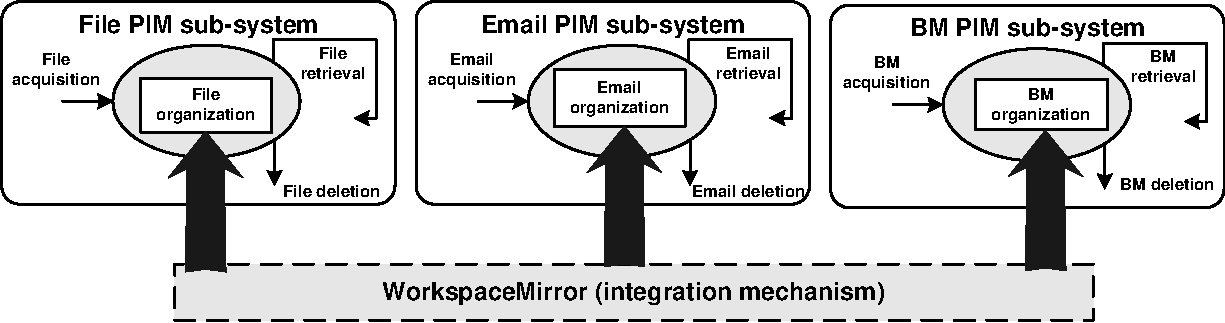
\includegraphics[width=.9 \textwidth]{pictures/discussion/PIM-cross-tool-artefact.pdf}
		% fs-fm-comparison.pdf}
	\end{center}
	\caption{WorkspaceMirror conceptualized as a cross-tool artefact which acts as a design intervention in multiple PIM-tools}
	\label{fig:discussion:ct-artefact}
\end{figure}

% Cross-tool scenarios, as discussed above, may be useful in identifying unforeseen impacts.


% This thesis is a case-study in doing just this.
% uch recommendations are only useful if its influences practice.  
% operationalize
% Rest of thesis is an exercise in putting these methodological suggestions into practice.  This thesis as putting such a cross-tool perspective into operationalization.  Leading into the practical and analytical work to follow, the operationalization of this methodology.
This thesis acts as a case-study to illustrate how many of these recommendations can be put into practice. \textbf{Chapter~\ref{chapter:exploratory_study}} reported a cross-tool study which surveyed user behaviour across files, email and bookmarks.  \textbf{Chapter~\ref{chapter:design}} reported a cross-tool design and implementation based on those requirements. \textbf{Chapter~\ref{chapter:main-study}} reported the cross-tool evaluation of the design.

%%%%%%%%%%%%%%%%%%%%%%%%%%%%%%%%%%%%%%%%%%%%%%%%%%%%%%%%%%%%%%%%%%%%%%%%%%%%%%%%%%%%%%%%%%%%%%%%%%%%%%%%%%%%%%%%%
%%%%%%%%%%%%%%%%%%%%%%%%%%%%%%%%%%%%%%%%%%%%%%%%%%%%%%%%%%%%%%%%%%%%%%%%%%%%%%%%%%%%%%%%%%%%%%%%%%%%%%%%%%%%%%%%%
%%%%%%%%%%%%%%%%%%%%%%%%%%%%%%%%%%%%%%%%%%%%%%%%%%%%%%%%%%%%%%%%%%%%%%%%%%%%%%%%%%%%%%%%%%%%%%%%%%%%%%%%%%%%%%%%%
%%%%%%%%%%%%%%%%%%%%%%%%%%%%%%%%%%%%%%%%%%%%%%%%%%%%%%%%%%%%%%%%%%%%%%%%%%%%%%%%%%%%%%%%%%%%%%%%%%%%%%%%%%%%%%%%%

%%%%%%%%%%%%%%%%%%%%%%%%%%%%%%%%%%%%%%%%%%%%
\subsection{Designing for an Ongoing Activity}
\label{discussion:methodology:ongoing}
%%%%%%%%%%%%%%%%%%%%%%%%%%%%%%%%%%%%%%%%%%%%
%%%%%%%%%%%%%%%%%%%%%%%%%%%
% USE IN METH RECS
% (1) IMPLICS FOR EVAL
% (2) IMPLICS FOR STUDY
%%%%%%%%%%%%%%%%%%%%%%%%%%%

\textbf{Section~\ref{discussion:ongoing}} detailed two longitudinal perspectives from which PIM can be analysed: (1) as a sequence of discrete events, and (2) as a ongoing activity.  Here it is argued that both perspectives can be useful during requirements gathering and evaluation:
 
% Interface design and evaluation: must consider short-term and long-term needs and scenarios.
% In the short-term, efficiency of one-off events may be more important. However, over the long-term satisfaction may be more important based on the long-term perspective.  In the extreme, the lifetime of personal information now extends over the life-time of an individual.  Also the middle ground of acquisition/retrieval pairs and possible interference between them.  
% Consideration of user requirements on both time-scales is encouraged.
\begin{itemize}

\item \textit{Requirements gathering} -- Attention should be paid to both time-scales when assessing user needs.  For example, user needs in the short-term may conflict with those in the long-term. As well as analysing interactions as one-off events, the impact of a design intervention on associated events, such as storage and retrieval, should be considered.   For example, consider the design of a new search mechanism.  In the short-term, the optimization of the efficiency of a discrete individual retrieval event may be paramount.  However, over the long-term, users may want to reuse search requests. This would suggest the need to save and possibly organize those requests. This in turn may increase the time and complexity in making the initial request.

%%%%%%%%%%%%%%%%%%%%%%%%%%%%%%%%%%%%%%%%%%%%%%
% Consider the different PIM sub-activities
%%%%%%%%%%%%%%%%%%%%%%%%%%%%%%%%%%%%%%%%%%%%%%
One useful approach may be to employ a scenario centred on the \textit{life-cycle of a piece of information}.  Tracking interactions with a particular piece of information over time may highlight user issues in terms of a sequence of PIM actions involving all the PIM sub-activities.  
% PIM constitutes a range of sub-activities: acquisition, organization, maintenance, and retrieval.  Therefore, user needs may vary depending on \textit{both} time-scale and sub-activity.  

%%%%%%%%%%%%%%%%%%%%%%%%%%%%%%%%%%%%%%%%%%%%%%%%%%%%%%%%%%%%%
%%%%%%%%%%%%%%%%%%%%%%%%%%%%%%%%%%%%%%%%%%%%%%%%%%%%%%%%%%%%%
%%%%%%%%%%%%%%%%%%%%%%%%%%%%%%%%%%%%%%%%%%%%%%%%%%%%%%%%%%%%%
%%%%%%%%%%%%%%%%%%%%%%%%%%%%%%%%%%%%%%%%%%%%%%%%%%%%%%%%%%%%%
%%%%%%%%%%%%%%%%%%%%%%%%%%%%%%%%%%%%%%%%%%%%%%%%%%%%%%%%%%%%%
% ONGOING: DESIGN IMPLICATIONS
%%%%%%%%%%%%%%%%%%%%%%%%%%%%%%%%%%%%%%%%%%%%%%%%%%%%%%%%%%%%%
Some user needs may only be apparent over the long-term.  For instance, the folder hierarchy is often criticized for not being easily adaptable to fast-changing user needs.  Consequently, requirements for dynamic views of personal information are often emphasized in PIM design, e.g.~\citep{dourish:99a,Dumais:03a}.  A long-term perspective may suggest a contrasting view: that the slow-changing nature of the folder hierarchy may
benefit users by promoting familiarity with the personal information environment. Such familiarity in turn supports location-based finding for which users expressed a clear preference.  Thus, \textit{persistence} is highlighted as an often overlooked, yet desirable design goal.  % Current tools, by their static nature, are good at supporting this design goal.


%%%%%%%%%%%%%%%%%%%%%%%%%%%%%%%
% Evaluate over long-term.  
%%%%%%%%%%%%%%%%%%%%%%%%%%%%%%%
% Participants can take a long time to adjust strategy with a background activity like PIM.  
% Also, first impressions may not reflect long-term behaviour.  In the main study both F3 and M5 changed their mind regarding their opinion of the WM prototype.
\item \textit{Evaluation} -- Evaluation should be performed over the long-term.  The fact that several participants changed their opinion regarding the WM prototype in \textbf{Chapter~\ref{chapter:main-study}} emphasises this point.  Such key observations would not have been revealed in a ``snapshot'' study.  Furthermore, the incremental nature of strategy changes, as reported in \textbf{Chapter~\ref{chapter:main-study}}, means that it may take time for users to adapt to new tools and for stable behaviour to emerge.  % If possible, give users time to adapt their behaviour evolve. % Users may change slowly (especially if don't want to press-gang and bias them).

\end{itemize}

%%%%%%%%%%%%%%%%%
% theory crap
%%%%%%%%%%%%%%%%%
% The theory (UXP model and change/settled model): step towards modelling over long-term, strategy evolution.  Future work: Models exist for short-term IR events.  What about 
%DEVELOPING THEORY:  Theory: step towards modelling over long-term.  UXP
% Most theoretical models relate to the modelling of short-term events.  % is this true for balter? Here, the importance of developing models over the long-term is stressed, such modelling as storage/retrieval event sequences related to one piece of information.  
% Later in this chapter, two long-term models are offered as indications of the kind of work which could usefully be done.  Firstly, a model of strategy changes over time is presented in \textbf{Section X}. Also, a model of user experience over time is presented in \textbf{Section~\ref{discussion:uxp}}.



%%%%%%%%%%%%%%%%%%%%%%%%%%%%%%%%%%%%%%%%%%%%%%%%%%%%%%%%%%%%%%%%%%%%%%%%%%%%%%%%%%%%%%%%%%%%%%%%%%%%%%%%%%%%%%%%%
%%%%%%%%%%%%%%%%%%%%%%%%%%%%%%%%%%%%%%%%%%%%%%%%%%%%%%%%%%%%%%%%%%%%%%%%%%%%%%%%%%%%%%%%%%%%%%%%%%%%%%%%%%%%%%%%%
%%%%%%%%%%%%%%%%%%%%%%%%%%%%%%%%%%%%%%%%%%%%%%%%%%%%%%%%%%%%%%%%%%%%%%%%%%%%%%%%%%%%%%%%%%%%%%%%%%%%%%%%%%%%%%%%%
%%%%%%%%%%%%%%%%%%%%%%%%%%%%%%%%%%%%%%%%%%%%%%%%%%%%%%%%%%%%%%%%%%%%%%%%%%%%%%%%%%%%%%%%%%%%%%%%%%%%%%%%%%%%%%%%%

%%%%%%%%%%%%%%%%%%%%%%%%%%%%%%%%%%%%%%%%%%%%
\subsection{Designing for a Supporting Activity}
\label{discussion:methodology:supporting}
%%%%%%%%%%%%%%%%%%%%%%%%%%%%%%%%%%%%%%%%%%%%

%  due to the provision of information needs by higher-level production activities. 
\textbf{Section~\ref{discussion:supporting}} discussed how PIM is not a self-contained activity.  Instead, it is driven by the production activities which provide the user's information needs.   Such a view suggests that the evaluation of PIM technology should not be limited to measuring improvements in the context of PIM alone.  The effectiveness of how well that PIM-tool supports production activities, may be a useful measure of tool effectiveness. % should also be considered, as well as measures of ongoing user satisfaction.
However, the author notes that such indirect measures of design success may be hard to capture in practice.
% Cross-tool production activities that involve multiple PIM-tools (e.g. starting a major project) may be useful approaches to investigating user requirements from a cross-tool perspective.  They may also be useful in guiding the evaluation of integration designs.

%%%%%%%%%%%%%%%%%%%%%%%%%%%%%
% STUDY:NATURE:SUPPORTING
%%%%%%%%%%%%%%%%%%%%%%%%%%%%%
% for example to help them optimize their PIM strategies
The author also observes that the very notion of PIM as a supporting activity leads to a dilemma for the designers of PIM-tools. As a supporting activity, PIM can both help and hinder production activities.  More time spent on PIM may result in better strategies and higher productivity.  However, there may be a very different consequence of spending more time managing information: distraction from the very production activities that PIM supports. %   -- however, too much PIM may in fact distract the user from what they are meant to be doing.
%\textbf{Section~\ref{discussion:uxp-balance}} describes the implications of PIM's supporting nature for PIM-tool designers, and employers alike.

\begin{itemize}

\item \textit{Encouraging users to spend more time on PIM} -- During the main study, participants reported that they were more focused on PIM due to the author's study and design interventions.  Those participants who changed strategies noted that this increased focus was a key factor in helping them optimize their management style. Although the changes observed in the main study were subtle, participants found them beneficial.  % This suggests that users may benefit from increased reflection on PIM.  

%%%%%%%%%%%%%%%%%%%%%%%%%%%%%%%%%%%%%%
% TO ADD: IMPLICATIONS FOR DESIGNERS
%%%%%%%%%%%%%%%%%%%%%%%%%%%%%%%%%%%%%%
% Encouraging reflection. 
%\item As an alternative to redesigning tools to promote reflection (e.g. providing statistics on time spent filing and searching), organizations could also play a part here. Typically, organizations are more concerned with knowledge management and other strategic IT - whilst PIM is left to the individual. Nevertheless, PIM is a key aspect of employees' activities and has the potential to cause frustration and waste time. Organizations could publicize PIM-related issues, and encourage employees to self-diagnose problems to improve their PIM effectiveness. (DESIGN RECS)
This suggests a potential design route: encourage users to devote more attention to PIM, so they can improve their strategies, and receive the same benefits that resulted from the ``self-auditing'' effect of the study.  As an alternative to redesigning tools to promote reflection (e.g. providing statistics on time spent filing and searching), organizations could also play a part here. Typically, organizations are more concerned with knowledge management and other strategic IT -- whilst PIM is left to the individual.  Nevertheless, PIM is a key aspect of employees' activities and has the potential to cause frustration and waste time.  Organizations could publicize PIM-related issues, and encourage employees to self-diagnose problems to improve their PIM effectiveness.  There may even be a case for PIM training days to recommend guidelines for effective PIM, e.g.~\citep{Allen:03}.  However, managers  should take care not to be overly prescriptive, or they may be seen to be interfering with individuals' preferred style. 
% Which of these people could benefit from increased reflection? 

% \textbf{Section~\ref{main-study:results:reflection}} participants feedback on the pros and cons of increased reflection on PIM.  

\item \textit{The downsides of spending too much time on PIM} -- Some main study participants also noted the downsides of paying increased attention to PIM: that less attention is available for other activities. This raises a challenge for users, managers and designers alike -- they must help the user to \textit{balance} PIM and the production activities that it supports.

The dilemma for PIM-tool designers is discussed further as follows.  Several of the main study participants gave examples of how ticking off to-do items or filing email messages could be highly satisfying, and even act as a therapeutic break from ``real work''.    One can envisage a PIM-tool that is so effectively designed and so satisfying to use, that its users spend all their time managing the information it contains.  Should designers be encouraging users to spend more time on PIM?   Although this may have the benefit of helping the user improve their strategies, there may also be associated costs.  Every extra minute spent on PIM, is a minute taken away from production activities.  A key challenge for designers is to help users find their ``balance point''.  Designers should encourage users to do enough PIM to support their production activities, but not so much to cause distraction from them.

\end{itemize}



% users may benefit from increased attention to PIM, for example to help them optimize their PIM strategies. Such an increase was manifested in the design and study interventions performed in the main study.  
%Lack of reflection (related to changes in strategy observed in main study).
% ADD: Generally people changed slowly







%  (user needs to do enough PIM to support his/her needs, ie. need to be ``active'').  

% This may be ensuring backups are taken (should be automatic of course).
% Relate to design recommendation relating to promotion of reflection

% So is the ultimate PIM-tool one which is totally transparent -- Star Trek computer meets google?
%%%%%%%%%%%%%%%%%%%%%%%%%%%%%%%%%%%%%%%%%%%%%%%%%%%%%%%%%%%%%%%%%%%%%%%%%%%%%%%%%%%%%%%%%%
% The next section moves on to discuss PIM from a second theoretical perspective, that of a \textit{cross-tool} activity.
% \textit{LINK: Used in UXP section}


%%%%%%%%%%%%%%%%%%%%%%%%%%%%%%%%%%%%%%%%%%%%%%%%%%%%%%%%%%%%%%%%%%%%%%%%%%%%%%%%%%%%%%%%%%%%%%%%%%%%%%%%%%%%%%%%%
%%%%%%%%%%%%%%%%%%%%%%%%%%%%%%%%%%%%%%%%%%%%%%%%%%%%%%%%%%%%%%%%%%%%%%%%%%%%%%%%%%%%%%%%%%%%%%%%%%%%%%%%%%%%%%%%%
%%%%%%%%%%%%%%%%%%%%%%%%%%%%%%%%%%%%%%%%%%%%%%%%%%%%%%%%%%%%%%%%%%%%%%%%%%%%%%%%%%%%%%%%%%%%%%%%%%%%%%%%%%%%%%%%%
%%%%%%%%%%%%%%%%%%%%%%%%%%%%%%%%%%%%%%%%%%%%%%%%%%%%%%%%%%%%%%%%%%%%%%%%%%%%%%%%%%%%%%%%%%%%%%%%%%%%%%%%%%%%%%%%%


%%%%%%%%%%%%%%%%%%%%%%%%%%
% \subsection{Summary}
%%%%%%%%%%%%%%%%%%%%%%%%%%
% Lessons which other researchers can take away ...
% Also can consider basing recommendations on nature of PIM (theory), and based on that derive methodological mplications
% Consider separate section with all recommendations collated. 
% SUMMARY POINT: trying to deal with poor epistemic state of PIM/HCI (anti revolutionary design, research-practice gap)
% This section made a number of methodological recommendations. These are used to drive the directions for future work suggested in \textbf{Chapter~\ref{chapter:conclusion}}.


%%%%%%%%%%%%%%%%%%%%%%%%%%%%%%%%%%%%%%%%%%%%%%%%%%%%%%%%%%%%%%%%%%%%%%%%%%%%%%%%%%%%%%%%%%%%%%%%%%%%%%%%%%%%%%%%%
%%%%%%%%%%%%%%%%%%%%%%%%%%%%%%%%%%%%%%%%%%%%%%%%%%%%%%%%%%%%%%%%%%%%%%%%%%%%%%%%%%%%%%%%%%%%%%%%%%%%%%%%%%%%%%%%%
%%%%%%%%%%%%%%%%%%%%%%%%%%%%%%%%%%%%%%%%%%%%%%%%%%%%%%%%%%%%%%%%%%%%%%%%%%%%%%%%%%%%%%%%%%%%%%%%%%%%%%%%%%%%%%%%%
%%%%%%%%%%%%%%%%%%%%%%%%%%%%%%%%%%%%%%%%%%%%%%%%%%%%%%%%%%%%%%%%%%%%%%%%%%%%%%%%%%%%%%%%%%%%%%%%%%%%%%%%%%%%%%%%%

